\documentclass[FM,BP]{tulthesis}
\usepackage{tul}
\usepackage[czech]{babel}
\usepackage[utf8]{inputenc}
\usepackage[LY1,T1]{fontenc}
\usepackage[utf8]{inputenx}
\usepackage[nottoc]{tocbibind}
\usepackage{graphicx}
\usepackage{parskip}
\usepackage{subfig}
\usepackage{xparse,newunicodechar}
\usepackage{natbib}
\bibliographystyle{unsrt}


\TULtitle{Bezdrátové řízení motorů}{Wireless Control of motors}
\TULprogramme{B 2646}{Informační technologie}{Information technology}
\TULbranch{1802R007}{Informační technologie}{Information technology}
\TULauthor{Lukáš Souček}
\TULsupervisor{Ing. Lenka Kosková Třísková}
\TULyear{2018}
\begin{document}

\ThesisStart{male}
\begin{abstractCZ}
 
 
\end{abstractCZ}

\begin{abstractEN}


\end{abstractEN}

  
 
\tableofcontents

\clearpage


\begin{abbrList}
    RF & Radiofrekvenční \\
	Mhz & Megahertz \\
	Ghz & GigaHertz \\
\end{abbrList}



\chapter{Úvod}

\chapter {Systém Arduino}
Arduino je Hardware platforma umožňující pomocí softwaru v počítači vytvářet různé elektronické projekty nahráním vytvořeného kódu na desku. Pro připojení k počítači na kterém se obvykle programuje je třeba USB kabel, který zároveň slouží jako napájecí prvek. Programovací jazyk speciálně pro Arduino je jakousi zjednodušenou verzí jazyku C++, ale využít lze i ostatní volně dostupný software.\cite{internet}
\section {Vlastnosti}
Jednou z podstatných vlastností systému Arduino je jeho portabilita, kdy lze vytvořený projekt či program spustit na rozličných systémech ať už jde o Linux, Windows či Macintosh OSX. Levné součástky patří také k významným přednostím této platformy, v porovnání s jinými mikrokontroléry než je Arduino se cena pohybuje i pod cenou menší než je 1000 Kč. Jednoduché programovací prostředí je lehce pochopitelné pro začátečníky, ale umožňuje i docílení rozsáhlých projektů pokročilým programátorům. Dalším privilegiem je license Creative Commons u Arduino modelů, která poskytuje zcela zdarma vytvoření vlastní verze Arduino modulu i s několika vylepšeními navíc bez právních omezení.
\cite{arduino}
\section {Využití}
Samotná platforma Arduino nabízí spousty forem využití ať už jako jednoduchý systém umožňující snímat venkovní teplotu za pomoci různých senzorů připojených k Arduinu či obyčejný vysílač streamující televizní vysílání, tak také jako součást databázové technologie umožňující vysílat pokyny na desku, viz. část praktické části mé bakalářské práce.
\chapter {Aktuální bezdrátové technologie}
V této kapitole se poohlédnu po aktuální situaci v oblasti bezdrátových technologiích u platformy Arduino, jejich vlastnostech, možnostech reálného využití a jejich srovnáním se rozhodnu pro vhodnost určité technologie pro praktickou část.


\section {Bluetooth}
Technologie bluetooth využívající frekvence v rozmezí od stovek Mhz až po jednotky Ghz zpravidla s omezenou vzdáleností dosahu se dá jednoduše využít pro jednoduchý bezdrátový přenos mezi dvěma zařízeními Arduino či zabudovaným systémem bluetooth umožňující předávat získané výsledky z různých sensorů či v případě mé práce - motorů, zpět vysílací stanici.  S možností popasovat se s nepříliš velkou vzdáleností v dosahu se s pomocí modulu GSM zaobírá ve své práci (Reddy,2017) tým několika autorů pracující na frekvenci 800 Mhz ale i 1900 Mhz, vhodný pro příjem dat, připojení se provádí USART technologií. Se správným nastavením antény, kterou lze vidět na obrázku  se může docílit maximální vzdálenosti 35 km, což by stačilo pro naše potřeby, zanedbatelná je také cena, která se pohybuje v řádu několika stovek u nejnižších dosahů.

 
\section {Wi-fi}
Bezdrátový přenos za pomocí Wi-fi na frekvenci 2.4 Ghz ale i 5 Ghz.  Nejzásadnějším problémem je jakým způsobem se dá zajistit patřičné vysílání signálu, když se většinou přijímá. Podobně jako u radiové technologie se nejprve pošle kontrolní signál pro ověření, zda je systém připraven. O této možnosti se pojednává u (Aneiba 2014),který popisuje ovládání robotické ruky. V porovnáním s Bluetooth je odezva rychlejší i při větší vzdálenosti od daného Wi-fi zařízení, jak lze vidět na obrázku poukazující na nízké odezvy i v desítkách metrů.
\begin{figure}
	\begin{center}
		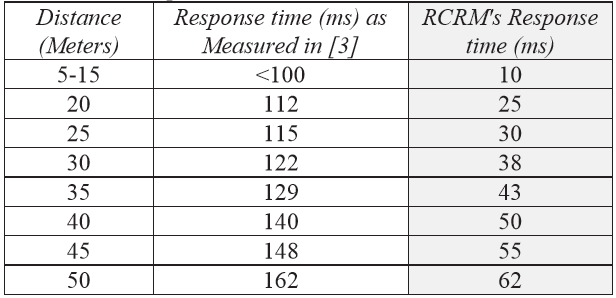
\includegraphics[scale=1.0]{Wifirange.png}
		\caption{Wifi latency}
		\label{Bluetooth}
	\end{center}
\end{figure} 

\section{Xbee}
Xbee je rádio podporující několik komunikačních protokolů (Zigbee či třeba Wifi),
možná varianta poskytující vysílání z bodu do bodu ale zároveň i smíšenou topologii umožňující využít vysílací prvek jako router, podobnou problematiku řeší (Kumbhar 2016), který pojednává o hlavním uzlem (routru) a dvěma senzory která předávají data hlavnímu uzlu. Opačného efektu chci dosáhnout ve své práci, směr, kterým se komunikuje je patrný z obrázku, kdy náš vysílač bude naopak řídit motory a posílat jim instrukce.Bezdrátové sítě se zpravidla skládají z uzlů, které navzájem pospolu komunikují. Kumbhar následně dokazuje reálnost využití Xbee modulu u sítí typu WSN - Ad-hoc síť, která integruje komunikaci v malých baterii napájených zařízeních, zmíněné uzly jako sensory spolupracují v rámci doručení požadovaných dat na správná místa. to umožňuje číst a snímat ku příkladu i potřebné krokové či servomotory. Na obrázku je vidět použitou komunikaci opačného formátu než by měla být ta má. \ref{System}
\cite{7860081}

\begin{figure}
	\begin{center}
		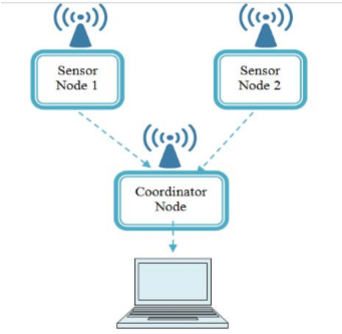
\includegraphics[scale=1.0]{System.png}
		\caption{Design Systému}
		\label{System}
	\end{center}
\end{figure} 
\section {Rádio}
 
\chapter {Praktické využití RF technologie}
V této části ve zaobývám reálnou možností využít radiovou technologi jako příjímací a vysílací stane a jejího možného sestavení na základě požadavků, které jsem si vytyčil na počátku mé práce. Ze všech existujících technologií mě tato oslovila, jelikož nemá tak velký rušivý element v závislosti na menší využité vzdálenosti (desítky metrů)
 \cite{radio}
 \section {Vysílací a přijímací stanice}
  Modul rádia, jak přijímač tak i vysílač za cenu 100 Kč byl použit na komunikaci mezi 2 zařízeními Arduino, tato dvě malá udělátka stačilo napasovat na Datové piny, napájení a zem pro obsloužení obou stanic dle jednotlivých vlastostí, viz obrázek
  \subsection {Popis}
  \subsection {Funkce}
  \subsection {Schéma}
  \section {Motory}
  \subsection {Zapojení}
  \subsection {Stavový diagram}
\chapter {Webová aplikace}
\section {Funkce}
 \section {Použité moduly}
  \section {Zdrojový kód}
  
 
 
  
 

\bibliography{test}
\end{document}